\documentclass[../_main/handlingar.tex]{subfiles}

\begin{document}
\beslutsuppfoljning{Uppfräschning av Diplomat}

På vårterminsmötet 2016 beslutades att den gamla soffan och borden i Diplomat skulle slängas för att göra plats för nya soffor och bord. Denna förändring skulle skapa fler studie- och matplatser samtidigt som rummet inte skulle tappa sin funktion som filmvisningsrum. Arbetet skulle göras över sommaren och vara färdigt till nollningen till en kostnad av maximalt 25 000 kr.

Den gamla soffan och de gamla borden har slängts respektive blivit mikrovågshyllor. Den nya uppställningen med soffor och bord har skapat åtminstone 12 nya och bekväma studieplatser med bra studiebelysning. Rummet står sällan tomt vilket får tolkas som ett bra betyg. Rummet har inte använts till att visa filmer i samma utsträckning som innan renoveringen, vilket möjligtvis beror på att sektionens medlemmar inte tänker på att inventarierna i rummet kan flyttas runt och sofforna kan ställas längs väggarna och bygga upp formen av den gamla soffan.

Förutom de nya inventarierna har väggarna målats om och “projektorduken” tvättats för att ytterligare fräscha upp rummet. Budgeten på 25 000 kr har hållts.

Med anledning av ovanstående yrkar vi på

\begin{attsatser}
    \att stryka \emph{Uppfräschning av Diplomat} från beslutsuppföljningen.
\end{attsatser}

\emph{Resultatrapport finns på nästa sida.}

\begin{signatures}{1}
    \ist
    \signature{Johannes Koch}{ENU-ordförande 2016}
\end{signatures}

\newpage
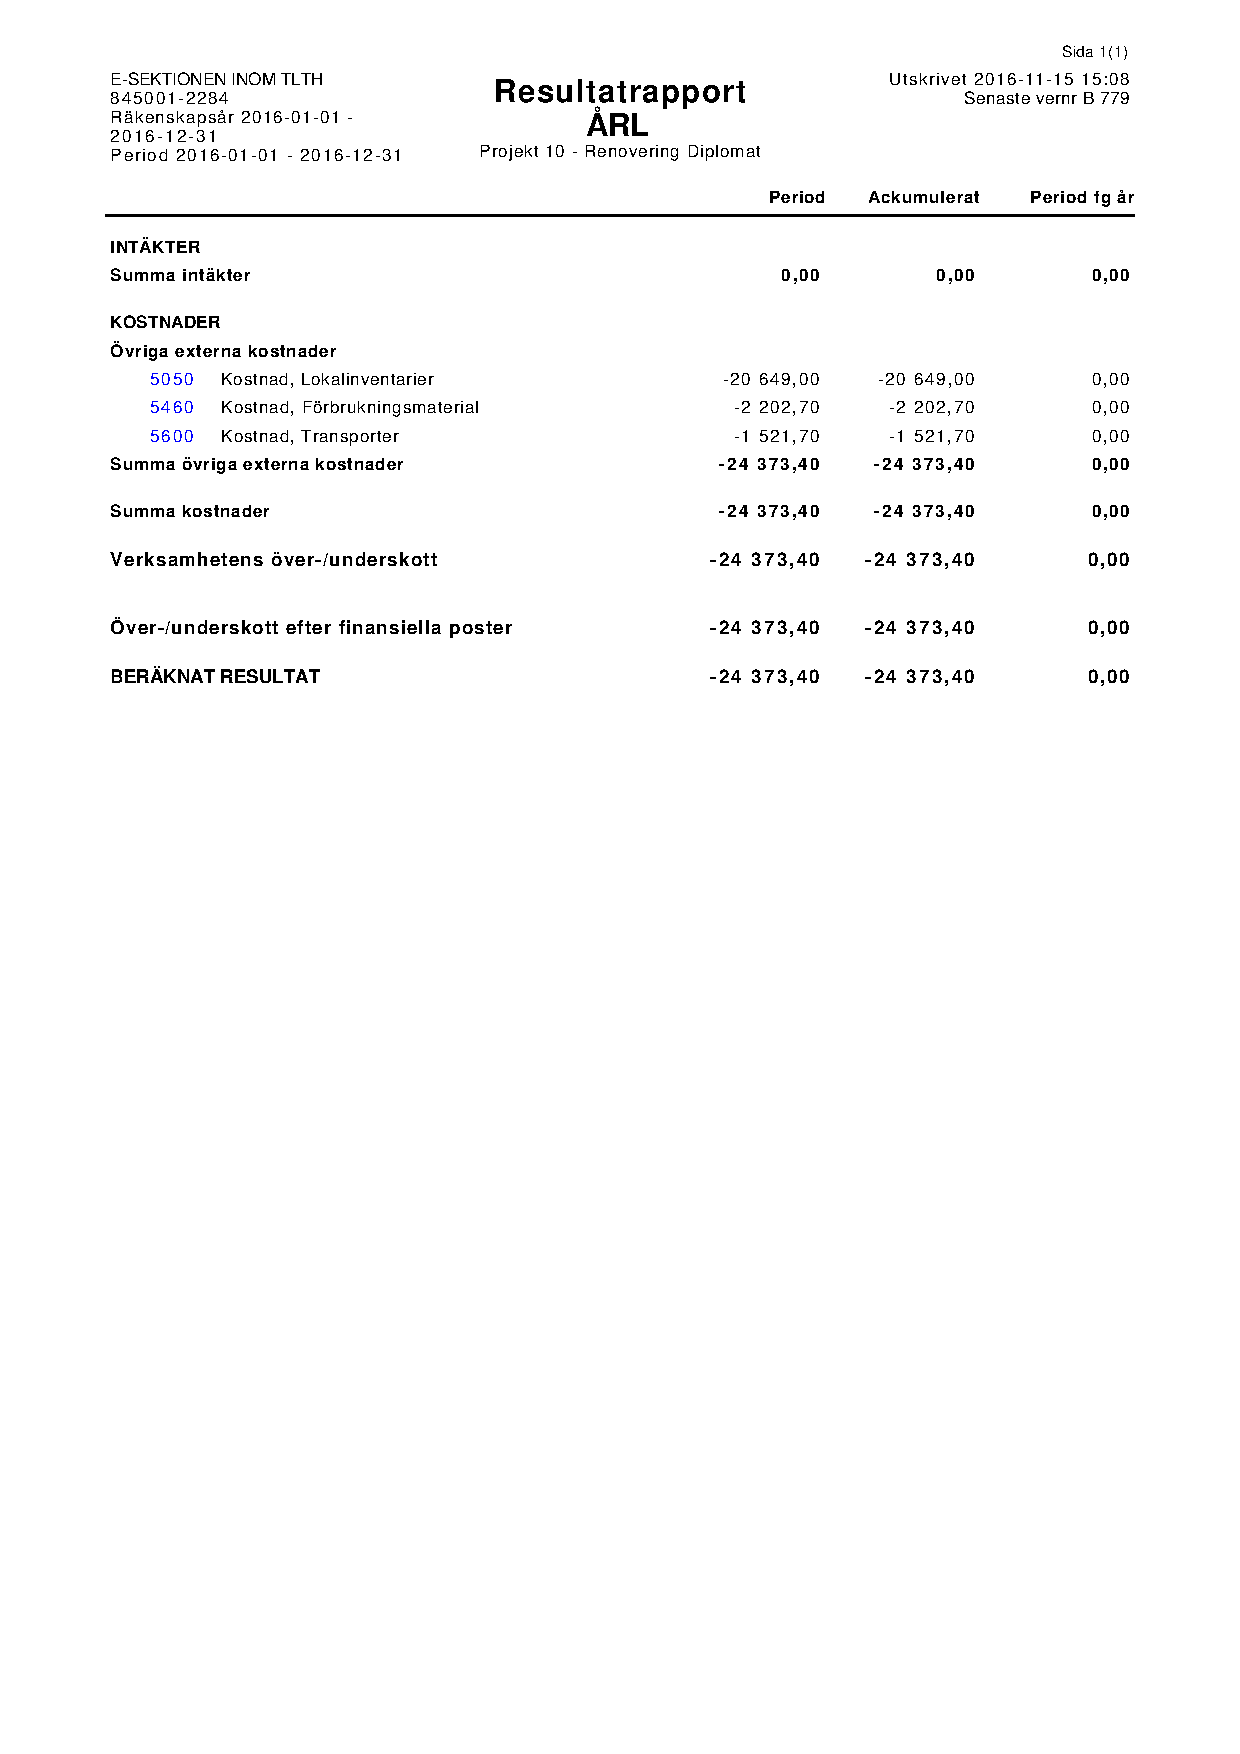
\includepdf[pages=-]{../_res/diplomat.pdf}


\end{document}
